% -*- TeX-master: "../dipole_ilya_paper.tex" -*-
\section{Dipole Transition}
\label{sec:dipole-transition}

We analyse  the tuneability  of the  \iket{2} \ra  \iket{1} transition  rate with
reference to Fermi's golden rule %\includeref{some shit}

 \begin{equation}\label{eqn:goldenRule}
   \frac{1}{T_{21}} = \frac{1}{Z_0}\hbar\omega_{21}\frac{\iabsSquared{\bra{2}T\iket{1}}}{\hbar^2}.
 \end{equation}

 \noindent The kinetic term $ T $ plays  the role of the dipole operator for this
 transition  and is  evaluated with  the  eigenstates \iket{1},  \iket{2} of  the
 Hamiltonian.   Highest  transition  rates  are achieved  around  the  degeneracy
 biases,     $    \varphi_{\text{ext}}     =    (2n+1)\pi,     n\in\mathbb{Z}    $,     see
 Fig.~\ref{fig:dipole_transition}. This region is thus favourable for quick state
 operations with external driving fields.
 
 \begin{figure}
   \centering 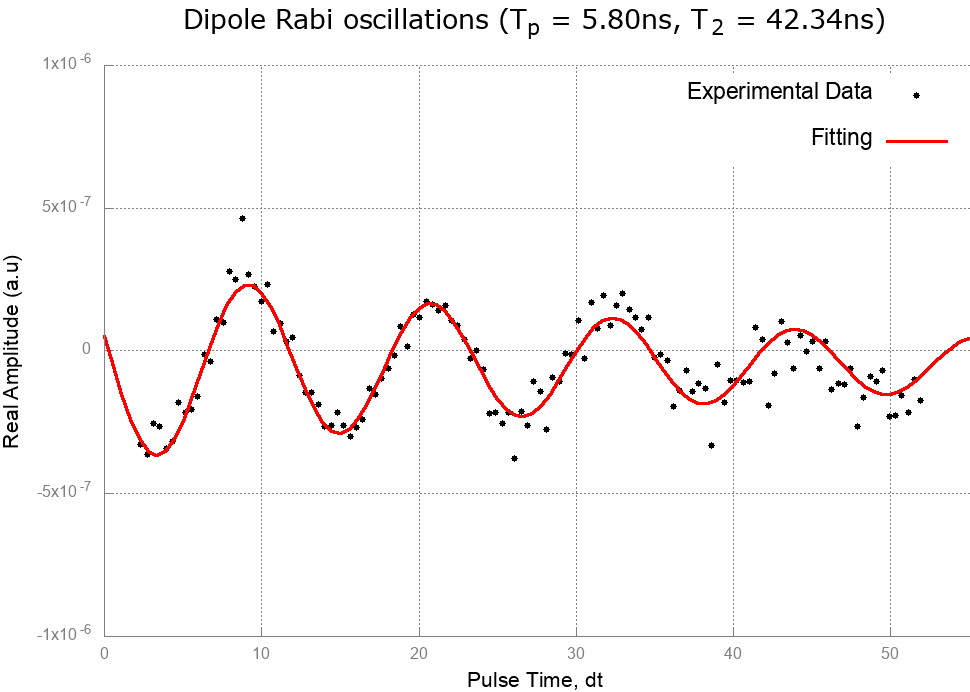
\includegraphics[height=6.5cm]{figure5.png}
 	\caption{The dipole transition rate $ \Gamma $ is proportional to the dipole transition element $ \bra{2}T\ket{1} $, where $ T $ is the charge operator responsible for the transition, and $ \iket{1} $ and \iket{2} are the eigenstates of the system. %There is strong transition between the levels at the turning point in magnetic flux, $ \Phi = (n+\frac{1}{2})\Phi_0, n\in\mathcal{Z} $.
          \label{fig:dipole_transition}}
      \end{figure}

%%% Local Variables:
%%% mode: latex
%%% TeX-master: "../dipole_ilya_paper"
%%% End:
